\documentclass[]{article}

% Imports the catppuccin theme, using the mocha flavor,
% from the directory above. Actual implementation
% wouldn't need the import package unless the theme
% and the document are in different directories.
\usepackage{import}
\usepackage{xcolor}
% \usepackage{fancyhdr}
\usepackage{cancel}
\usepackage{mathtools}

% For permutations and combinations
\newcommand\Myperm[2][^n]{\prescript{#1\mkern-2.5mu}{}P_{#2}}
\newcommand\Mycomb[2]{\prescript{#1\mkern-0.5mu}{}C_{#2}}

% Colors
\definecolor{yorhabg}{HTML}{FFFFFF}
\definecolor{yorhafg}{HTML}{000000}
\definecolor{yorhagrid}{HTML}{B5AF9C}
\definecolor{mred}{HTML}{D67069}
\definecolor{mblue}{HTML}{6887A1}

\pagecolor{yorhabg}
\color{yorhafg}

\usepackage{preamble}

% Removes padding above title
\usepackage{titling}
\setlength{\droptitle}{-10em}

% Font package
\usepackage[T1]{fontenc}

\usepackage{fouriernc}

\usepackage{sectsty}
\usepackage{graphicx}
\usepackage{amsmath}
\usepackage{amsfonts}
\usepackage{amssymb}
\usepackage[skins, most]{tcolorbox}
\usepackage{enumitem}

\DeclareMathOperator{\sgn}{sgn}

\usepackage{tikz}
\usepackage{eso-pic}
\usetikzlibrary{calc,shadows.blur}
\usetikzlibrary{angles, quotes}
\usetikzlibrary{3d}

% Margins
\topmargin=0in
\evensidemargin=0in
\oddsidemargin=0in
\textwidth=6.5in
\textheight=9.0in
\headsep=0.25in

\AtBeginEnvironment{tcolorbox}{\small}

\newtcolorbox{imp}{enhanced,arc=0mm,colback=yorhabg,colframe=mred,leftrule=10mm,coltext=yorhafg,%
overlay={\node[anchor=west,outer sep=2pt] at (frame.west) {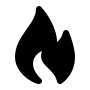
\includegraphics[width=6mm]{images/imageb.png}}; }}

\newtcolorbox{shortcut}{enhanced,arc=0mm,colback=yorhabg,colframe=mred,leftrule=10mm,coltext=yorhafg, coltitle=yorhabg, title=\texttt{Shortcut.}, 
overlay={\node[anchor=west,outer sep=2pt] at (frame.west) {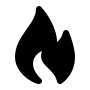
\includegraphics[width=6mm]{images/imageb.png}}; }}

\newtcolorbox{question}[1]{
    enhanced, 
    colback=yorhabg,
    colframe=mblue,
    coltext=yorhafg,
    coltitle=yorhabg,
    attach boxed title to top left={yshift*=-\tcboxedtitleheight}, 
    title=\texttt{#1},
    boxed title size=title,
    boxed title style={%
        rounded corners=northeast, 
        rounded corners=northwest, 
        colback=tcbcolframe, 
        boxrule=0pt,
    },
    underlay boxed title={%
        \path[fill=tcbcolframe] (title.south west)--(title.south east) 
            to[out=0, in=180] ([xshift=5mm]title.east)--
            (title.center-|frame.east)
            [rounded corners=5pt] |- 
            (frame.north) -| cycle; 
    },
}
% \pagestyle{fancy}
% \fancyhf{}  % Clear all default header/footer
% \fancyhead[L]{\small Satyajit Datta \\ 1012033336}  % Top-left, small font
\newcommand\bb[1]{\textcolor{yorhafg}{\textbf{#1}}}

\title{\textbf{MATA31 - Assignment \#4}}
\author{ Satyajit Datta \\ 1012033336}
\date{\today}

\begin{document}

\maketitle

\begin{question}{A}
Consider the linear function
\[
f(x) = 3x + 1.
\]

We know intuitively that
\[
\lim_{x \to -1} f(x) = -2.
\]

\begin{enumerate}[label=\textbf{\Alph*.}]
    \item How close to $-1$ does $x$ have to be such that $f(x)$ differs from $-2$
    by less than $0.1$?
    \item How close to $-1$ does $x$ have to be such that $f(x)$ differs from $-2$
    by less than $0.01$?
    \item How close to $-1$ does $x$ have to be such that $f(x)$ differs from $-2$
    by less than $0.001$?
\end{enumerate}
\end{question}

\begin{center}
    $\forall \varepsilon > 0\;\exists\; \delta>0 \quad \text{s.t} \quad 
    0 < |x-(-1)| < \delta \Longrightarrow |3x+1 - (-2)|  < \varepsilon$
\end{center}

When solving the limit, we get $\delta = \frac{\epsilon}{3}$.

\begin{enumerate}[label=\textbf{\Alph*.}]
    \item If $\varepsilon = 0.1$, $x$ has to be within $0.1 \div 3 = 0.0\overline{3}$ of $-1$
    \item If $\varepsilon = 0.01$, $x$ has to be within $0.01 \div 3 = 0.00\overline{3}$ of $-1$
    \item If $\varepsilon = 0.001$, $x$ has to be within $0.001 \div 3 = 0.000\overline{3}$ of $-1$
\end{enumerate}

\begin{question}{B}
    Provide the formal definition of the limit
    \[
    \lim_{x \to a} f(x) = L
    \]
    in two ways: one using intervals and one using absolute value inequalities. Use this definition to prove that
    \[
    \lim_{x \to 3} (2x+4) = 10
    \]
\end{question}

\underline{\bf{Interval Definition}}

\[
    \forall \varepsilon > 0 \;\exists\;\delta > 0 \quad \text{s.t} \quad x \in(c - \delta, c)\cup(c, c+\delta)\Longrightarrow f(x) \in (L-\varepsilon, L+\varepsilon)
\]

\underline{\bf{Absolute value inequalities}}
\[
    \forall \varepsilon > 0\;\exists\; \delta>0 \quad \text{s.t} \quad 
    0 < |x-c| < \delta \Longrightarrow |f(x) - L|  < \varepsilon
\]

\hrule
\vspace{0.1in}
We will use the absolute value inequality definition to prove this limit.

Want to show: 
\[
    \forall \varepsilon > 0\;\exists\; \delta>0 \quad \text{s.t} \quad 
    0 < |x-3| < \delta \Longrightarrow |(2x +4) - 10|  < \varepsilon
\]

\underline{\bf{Proof.}}

\underline{Let} $\varepsilon > 0$ be arbitrary.

\medbreak

\underline{Choose} $\delta = \frac{\varepsilon}{2}$. Note $\delta > 0$.

\medbreak

\underline{Assume} $0 < |x-3| < \delta$. Then, 

\begin{align*}
    |(2x + 4) -10| &= |2x-6| 
        && \text{(by algebra)} \\[6pt]
    &= |2(x-3)| 
        && \text{(by algebra)} \\[6pt]
    &= |2||x-3| 
        && \text{(by properties of $|\cdot|$)} \\[6pt]
    &= 2|x-3| 
        && \text{(since $2>0$)} \\[6pt]
    &< 2\delta 
        && \text{(by assumption)} \\[6pt]
    &= 2\!\left(\tfrac{\varepsilon}{2}\right) 
        && \text{(by choice of $\delta$)} \\[6pt]
    &= \varepsilon 
        && \text{(by algebra).}
\end{align*}

As required to show $\blacksquare$.
\begin{question}{C}
    Provide the formal definition of the limit
    \[
    \lim_{x \to a^+} f(x) = \infty
    \]
    in two ways: one using intervals and one using absolute value inequalities. Use this definition to prove that
    \[
    \lim_{x \to 1^+} \frac{1}{x-1} = \infty
    \]
\end{question}


\underline{\bf{Interval Definition}}

\[
    \forall M > 0 \;\exists\;\delta > 0 \quad \text{s.t} \quad x \in(a, a+\delta)\Longrightarrow f(x) \in (0, \;M)
\]

\underline{\bf{Absolute value inequalities}}
\[
    \forall M > 0\;\exists\; \delta>0 \quad \text{s.t} \quad 
    0 < x-a < \delta \Longrightarrow f(x) >M
\]

\hrule
\vspace{0.1in}
We will use the absolute value inequality definition to prove this limit.

Want to show:
\[
    \forall M > 0\;\exists\; \delta>0 \quad \text{s.t} \quad 
    0 < x-1 < \delta \Longrightarrow \frac{1}{x-1} > M
\]


\underline{\bf{Proof.}}

\underline{Let} $\varepsilon > 0$ be arbitrary.

\medbreak

\underline{Choose} $\delta = \frac{1}{M}$

\medbreak

\underline{Assume} $0 < x-1 < \delta$. Then:

\begin{align*}
    x - 1  & < \delta
        && \text{(by algebra)} \\[6pt]
    \Longrightarrow x-1 &= \frac{1}{M} 
        && \text{(by our choice of $\delta$)} \\[6pt]
    \Longrightarrow \frac{1}{x-1}  &> M
        && \text{(since $x > 0$ and $M > 0$)} \\[6pt]
\end{align*}

As required to show. $\blacksquare$.
\begin{question}{D}
    Provide the formal definition of the limit
    \[
    \lim_{x \to \infty} f(x) = L
    \]
    in two ways: one using intervals and one using absolute value inequalities. Use this definition to prove that
    \[
    \lim_{x \to \infty} \frac{2}{x+1} = 0
    \]
\end{question}

\underline{\bf{Interval Definition}}

\[
    \forall \varepsilon> 0 \;\exists\;N > 0 \quad \text{s.t} \quad x \in(0, \;N) \Longrightarrow f(x) \in (L -\varepsilon, \;L+\varepsilon)
\]

\underline{\bf{Absolute value inequalities}}
\[
    \forall \varepsilon > 0\;\exists\; N>0 \quad \text{s.t} \quad 
    x > N \Longrightarrow |f(x) - L| < \varepsilon
\]

\hrule
\vspace{0.1in}
We will use the absolute value inequality definition to prove this limit.
Want to show:

\begin{center}
    $\forall \epsilon > 0\;\exists\; N>0 \quad \text{s.t} \quad 
    x > N \Longrightarrow |\frac{2}{x+1} - 0| < \varepsilon$
\end{center}
\underline{\bf{Proof.}}

\underline{Let} $\varepsilon > 0$ be arbitrary.

\medbreak

\underline{Choose} $N = \max\{ 1, \frac{2}{\varepsilon} - 1 \}$. Note that $N > 0$.

\medbreak

\underline{Assume} $x > N$. Then

\begin{align*}
    x  & >\; \frac{2}{\varepsilon} - 1
        && \text{(by our choice of N)} \\[6pt]
    \Longrightarrow x+1 &=\; \frac{2}{\varepsilon}
        && \text{(by algebra)} \\[6pt]
    \Longrightarrow \frac{1}{x+1}  &<\; \frac{\varepsilon}{2}
        && \text{(since $x > 0$ and $\varepsilon > 0$)} \\[6pt]
    \Longrightarrow \frac{2}{x+1}  &<\; \varepsilon
        && \text{(by algebra)} \\[6pt]
    \Longrightarrow \frac{2}{x+1} - 0 &<\; \varepsilon
        && \text{(by algebra)} \\[6pt]
    \Longrightarrow |\;\frac{2}{x+1}\; - 0\;| &<\; \varepsilon
        && \text{(since $x > 0$)} \\[6pt]
\end{align*}


As required to show $\blacksquare$.
\begin{question}{E}
    Provide the formal definition of the limit
    \[
    \lim_{x \to \infty} f(x) = \infty
    \]
    in two ways: one using intervals and one using absolute value inequalities. Use this definition to prove that
    \[
    \lim_{x \to \infty} (x^2+1) = \infty
    \]
\end{question}

\underline{\bf{Interval Definition}}

\[
    \forall M > 0 \;\exists\;N > 0 \quad \text{s.t} \quad x \in(0, \;N) \Longrightarrow f(x) \in (0, \;M)
\]

\underline{\bf{Absolute value inequalities}}
\[
    \forall M > 0\;\exists\; N>0 \quad \text{s.t} \quad 
    x > N \Longrightarrow f(x) > M
\]

\hrule
\vspace{0.1in}
We will use the absolute value inequality definition to prove this limit.

Want to show: 
\[
    \forall M > 0\;\exists\; N >0 \quad \text{s.t} \quad 
    x > N \Longrightarrow x^2+1 > M
\]

\underline{\bf{Proof.}}

\underline{Let} $M > 0$ be arbitrary

\medbreak

\underline{Choose} $N = \sqrt{M} $. Note that N > 0.

\medbreak

\underline{Assume} $x > N$. Then


\begin{align*}
    x^2+1  & > N^2 + 1
        && \text{(by algebra)} \\[6pt]
    &= M+1 
        && \text{(by our choice of $N$)} \\[6pt]
    & > M
        && \text{(by properties of inequalities)} 
\end{align*}

As required to show $\blacksquare$.

\begin{question}{F}
    Find the equation of a possible function $f$ with $f(0) = 5, \displaystyle{\lim_{x\to1^+}} f(x) = \infty$ and $\displaystyle{\lim_{x\to1^-}} f(x) = \infty$
\end{question}

The equation that we will choose is:

\[
    f(x) = \frac{1}{(x-1)^2} + 4
\]

The reason I chose this function is because I know $\frac{1}{(x-1)^2}$ has an asymptote at $x = 1$, so I squared the denominator to make the function approach $+\infty$ on both sides.
The value of this function is 1 at $x=0$, so I then added $4$.

\medbreak 

\textbf{\underline{Prove f(0) = 5}}
\begin{align*}
    f(x) &= \frac{1}{(x-1)^2} + 4 \\
    f(\bf{0}) &= \frac{1}{(\bf{0}-1)^2} + 4 \\
    &= \frac{1}{(-1)^2} + 4 \\
    &= \frac{1}{1} + 4 \\
    &= 1 + 4\\
    &= 5 
\end{align*}

As required to show. $\blacksquare$.

\medbreak

The limit as $x \rightarrow 1$ is $\infty$, making each one-sided limit also $\infty$.


\begin{question}{G}
    Does
    \[
    \lim_{x \to 2} \frac{|x-2|}{x-2}
    \]
    exist? Explain why or why not.  
\end{question}

The numerator of this function is always positive, so we can disregard it, as the sign doesn't change whether $x \to 2^-$ or $x \to 2^+$. There is a vertical asymptote at $x = 2$. If $x < 2 \Rightarrow f(x) < 0$, and if $x > 2 \Rightarrow f(x) > 0$, Therefore the limit does not exist $\blacksquare$. 
\begin{question}{H}
    Find $\displaystyle{\lim_{x\to 3}} f(x)$ if it exists. Otherwise, explain by one-sided limits
    
    \[
        f(x) =
        \begin{cases}
            x^2, & \text{if } x \leq 3, \\
            3x + 2, & \text{if } x > 3.
        \end{cases}
    \]

\end{question}

Lets look at each piece individually.

\[
    \lim_{x\to3} x^2 = 9
\]

Let us prove this.

Want to show: 
\[
    \forall \varepsilon > 0\;\exists\;\delta >0 \quad \text{s.t} \quad 
    0 < |x-3| < \delta \Longrightarrow |x^2-9| < \varepsilon
\]

\underline{\bf{Proof.}}

\underline{Let} $\varepsilon > 0$ be arbitrary

\medbreak

\underline{Choose} $\delta = min\{1, \frac{\epsilon}{7}\} $. Note that N > 0.

\medbreak

\underline{Assume} $0 < |x-3| < \delta$.
\medbreak
Since $x^2 - 9 = (x+3)(x-3)$ and $x-3 < \delta$, we first need to obtain a bound on $|x+3|$. Then
\begin{align*}
    |x-3| < \delta &\Longrightarrow |x-3|<1
        && \text{(since $\delta = \min\{ 1, \frac{\varepsilon}{7} \} \le 1$)} \\[6pt]
    &\Longrightarrow -1 < x-3 < 1
        && \text{(by properties of $|\cdot|$)} \\[6pt]
    &\Longrightarrow 5 < x+3 < 7 
        && \text{(by algebra)} \\[6pt]
    &\Longrightarrow -7 < x+3 < 7
        &&\text{(by properties of inequalities)} \\[6pt]
    &\Longrightarrow |x+3| < 7
        &&\text{(by properties of $|\cdot|$)} \\[6pt]
\end{align*}

Therefore, $|x+3| < 7$ $(\star)$.

It now follows that:
\begin{align*}
    |x^2 - 9| &= |(x+3)(x-3)| 
        && \text{(by algebra)} \\[6pt]
    &= |x+3||x-3| 
        && \text{(by properties of $|\cdot|$)} \\[6pt]
    &< |x+3|\delta 
        && \text{(by assumption)} \\[6pt]
    &< 7\delta 
        && \text{(by ($\star$))} \\[6pt]
    &= 7\frac{\epsilon}{7} 
        && \text{(by our choice of $\delta$)} \\[6pt]
    &= \varepsilon 
        && \text{(by algebra).}
\end{align*}

As required to show. $\blacksquare$.
\vspace{0.1in}
\hrule
\vspace{0.1in}
Now, lets look at 
\[
    \lim_{x\to3} 3x+2 = 11
\]

Let us prove this.

Want to show: 
\[
    \forall \varepsilon > 0\;\exists\;\delta >0 \quad \text{s.t} \quad 
    0 < |x-3| < \delta \Longrightarrow |(3x+2)-11| < \varepsilon
\]

\underline{\bf{Proof.}}

\underline{Let} $\varepsilon > 0$ be arbitrary

\medbreak

\underline{Choose} $\delta = \frac{\epsilon}{3} $. Note that N > 0.

\medbreak

\underline{Assume} $0 < |x-3| < \delta$.

\begin{align*}
    |(3x + 2) -11| &= |3x-9| 
        && \text{(by algebra)} \\[6pt]
    &= |3(x-3)| 
        && \text{(by algebra)} \\[6pt]
    &= |3||x-3| 
        && \text{(by properties of $|\cdot|$)} \\[6pt]
    &= 3|x-3| 
        && \text{(since $2>0$)} \\[6pt]
    &< 3\delta 
        && \text{(by assumption)} \\[6pt]
    &= 3\frac{\varepsilon}{3}
        && \text{(by choice of $\delta$)} \\[6pt]
    &= \varepsilon 
        && \text{(by algebra).}
\end{align*}

As required to show. $\blacksquare$.

\vspace{0.1in}
\hrule
\vspace{0.1in}



Since the left sided limit $\ne$ the right sided limit, the limit does not exist. $\blacksquare$.
\end{document}